% =====================================================================
% From board to graph: a hybrid human-AI role-playing board for critical
% media and AI literacy
% Target: The International Journal of Games and Social Impact (IJGSI),
%         Vol. 5, No. 4 -- Games, Gamification, Media Literacy and
%         Transformation in Educational Contexts.
% Anonymised manuscript for double-blind review (author data go in the
% title page generated by word/folha_de_rosto.py). References: APA 7 via
% biblatex-apa. The journal accepts only Word/RTF: run `bash word/gerar.sh`.
% Figures 1 and 2 are TikZ sources in figuras/*.tex, rendered to PNG.
% =====================================================================
\documentclass[12pt]{article}

\usepackage[utf8]{inputenc}
\usepackage[T1]{fontenc}
\usepackage[english]{babel}
\usepackage{csquotes}
\usepackage{mathptmx}                      % Times, as the journal asks
\usepackage[a4paper,margin=2.54cm]{geometry}
\usepackage{setspace}\onehalfspacing
\usepackage{amsmath,amssymb}
\usepackage{graphicx}
\usepackage{booktabs}
\usepackage{tabularx}
\usepackage{fancyhdr}
\usepackage{xcolor}
\usepackage[hidelinks]{hyperref}
\usepackage[style=apa,backend=biber]{biblatex}
\addbibresource{referencias.bib}

\graphicspath{{figuras/}}

\pagestyle{fancy}\fancyhf{}\fancyhead[R]{\thepage}
\renewcommand{\headrulewidth}{0pt}

\title{\textbf{\textit{FROM BOARD TO GRAPH: A HYBRID HUMAN-AI ROLE-PLAYING BOARD FOR CRITICAL MEDIA AND AI LITERACY}}}
\author{[Anonymised for review]}
\date{}

\begin{document}
\maketitle
\thispagestyle{fancy}

\begin{abstract}
\noindent
Communities come to share one version of events through who is where, who
knows what and who controls central places. We present a role-playing board
on which students, alone or with generative-AI characters, can experience
and then inspect that process. The world is a grid, represented as a
matrix; a character can only build on events it saw or heard about; and the
causal links between events are drawn with yarn, so the story ends as a
visible graph. A simulation with synthetic agents shows that limiting
information only delays convergence to a single story, that central places
decide where stories merge, and that two mechanics keep several stories
alive. We describe the kit, a classroom protocol for critical media and AI
literacy, a low-tech version for contexts without devices, and an
evaluation plan.
\end{abstract}

\noindent\textit{Keywords: game-based learning; media literacy; AI literacy; role-playing games; board games; information disorder; network science}

% ---------------------------------------------------------------------
\section{Introduction}
% ---------------------------------------------------------------------

Every community tells itself stories about what happened: who was
responsible for a death, why the grain ran out, who is to blame for a debt.
Which of those stories survive is rarely a matter of evidence alone. It
depends on who was present, on who heard what from whom, and on who
controls the places where people meet. Accounts told at the periphery of
these networks are absorbed into the dominant one or never reach it. The
same mechanics operate, at a much larger scale, in the information
ecosystems that media literacy education is concerned with: rumours travel
along social ties, some places and channels concentrate attention, and a
shared account can form quickly around whatever happens to connect the most
people \parencite{wardle2017,hobbs2010}.

Games have proved to be good vehicles for teaching how such processes work.
Playing at producing misinformation, for instance, builds resistance to it
\parencite{roozenbeek2019,basol2020}, and games in general let learners
inhabit a system and reflect on its rules \parencite{gee2003,flanagan2009}.
Role-playing games add something specific: the story is co-created by the
participants as they play, so the process by which a shared account forms
is not only represented but enacted by the group itself
\parencite{fine1983,montola2008,bowman2010,daniau2016}.

Generative AI makes this both more urgent and more interesting. Language
models can now play characters in a shared world
\parencite{park2023,callisonburch2022}, and learners increasingly co-create
stories with them. A companion study, currently under review, simulated a
small town whose inhabitants were all language-model agents and recorded
every event with its declared causes. The storylines that appeared on the
second day of play merged into a single story within a few days, and they
merged along paths set by the premises of the world: characters whose
secrets referred to each other met first, in the places those secrets
named. One feature of that simulator matters for this paper: a single model
call decided what every character did and saw everything that had happened
recently, so the characters were effectively omniscient. In a tabletop game,
by contrast, players only know what their characters witnessed or were told.

This paper turns that contrast into a learning tool. We propose a
role-playing \emph{board} on which a small community lives: a grid of cells
with places, paths and a river; characters who can only build on what they
saw or heard; and event cards whose causes are tied together with yarn, so
that the story of the session ends as a physical graph on the table. The
same board can be played by people, by AI characters through a simulator,
or by mixed tables. The board is represented as a matrix, which lets us
reason about what its geometry does to the story with the tools of graph
theory, and test design options before taking them to a classroom.

The contributions are: (1) a formal model linking the board, the encounters
between characters and the causal graph of the story; (2) a proof of
concept with synthetic agents that identifies which mechanics change how
fast and where a shared story converges; (3) a physical kit and a hybrid
human--AI protocol; (4) a classroom protocol for critical media and AI
literacy, including a low-tech version; and (5) an evaluation plan. The
paper is a design and research proposal: the model and the simulation are
complete, the kit and the classroom protocol have not yet been tested with
learners.

% ---------------------------------------------------------------------
\section{Background}
% ---------------------------------------------------------------------

\subsection{Media literacy, information disorder and games}

Media literacy education asks learners to analyse who constructs messages,
how and with what effects \parencite{hobbs2010}. Information disorder
research has added a systemic view: false or misleading content matters less
as isolated items than as flows through networks of people, platforms and
places that amplify some accounts and silence others \parencite{wardle2017}.
AI literacy extends these questions to systems that generate content,
asking learners to understand what such systems can do, how they represent
the world and how their outputs are shaped \parencite{long2020,unesco2024}.
There is growing evidence that generative models homogenise what they help
to produce, from individual texts to plot elements
\parencite{doshi2024,padmakumar2024,xu2025,begus2024}.

Games have been used to teach these competences in two ways. Some games
simulate the production of misinformation so that players learn its
techniques from the inside, an approach that has measurable effects on the
ability to recognise manipulative content \parencite{roozenbeek2019,basol2020}.
Others use the procedural rhetoric of games, the way rules make an argument
\parencite{bogost2007}, to let players experience a social process and then
reflect on it \parencite{flanagan2009,flanagan2014}. The board proposed here
belongs to the second family. It does not teach players to recognise false
content; it lets a group experience how a shared account forms, and then
inspect the structure that produced it.

\subsection{Space, grids and social processes}

Game spaces tell stories by arranging places, paths and obstacles that
channel movement and encounters \parencite{jenkins2004}. Rules constrain the
fiction, and many rules are spatial \parencite{juul2005,salen2004}; modern
board games make these structures particularly legible
\parencite{woods2012}. Space syntax describes buildings and cities as graphs
and shows that the position of a space in that graph predicts how much it is
used and how people meet in it \parencite{hillier1984}. Grids have a long
history as minimal models of social processes, from segregation
\parencite{schelling1971} to whole artificial societies
\parencite{epstein1996} and cellular automata \parencite{wolfram1984}, and
they have been used in teaching precisely because they show collective
outcomes emerging from local structure without anyone intending them.

\subsection{Stories as graphs}

Narrative comprehension can be modelled as a causal network of events
\parencite{trabasso1985}; the kernels of a plot are the events with causal
antecedents and consequences \parencite{barthes1975,chatman1978}. Network
science supplies the tools to read such graphs: connected components,
bridges and articulation points \parencite{tarjan1972}, communities
\parencite{blondel2008}, time-respecting paths in networks whose links
appear and disappear \parencite{holme2012}, and the conditions under which a
growing graph becomes connected \parencite{newman2018}. Emergent narrative
research has long observed that autonomous agents produce events more
easily than stories with shape \parencite{aylett1999,louchart2004,riedl2013};
the companion study suggests that, with language-model agents, the problem
is the opposite of sprawl: everything connects.

% ---------------------------------------------------------------------
\section{Systematic literature review}
% ---------------------------------------------------------------------

We reviewed how analogue games have been used for media, information and AI
literacy, and how tabletop play has been combined with generative AI,
following the PRISMA 2020 reporting structure.

\paragraph{Search.} On 13 October 2026 we searched OpenAlex (title and
abstract), arXiv (abstract) and Semantic Scholar (bulk search) for records
from 2015 to 2026 that combine a game form (\enquote{board game},
\enquote{tabletop game}, \enquote{role-playing game}, \enquote{card game},
\enquote{tabletop role-playing}) with a literacy or AI term (\enquote{media
literacy}, \enquote{information literacy}, misinformation, disinformation,
\enquote{fake news}, \enquote{AI literacy}, \enquote{large language model},
\enquote{generative AI}). The exact strings, the raw responses and every
screening decision are in the supplementary material and in the public
repository.

\paragraph{Eligibility criteria.} Records were included when they met all of
the following: (I1) the study designs, uses or evaluates an analogue game
(board, card or tabletop role-playing game, including hybrid analogue-digital
versions), or a tabletop role-playing setting with generative AI; (I2) the
game targets media, information, news or AI literacy, misinformation or
critical thinking about information, or combines tabletop play with
generative AI; (I3) it is a peer-reviewed article, conference paper or
preprint in English, from 2015 to 2026. Records were excluded when the game
was not analogue or tabletop (E1), when it had no literacy or generative-AI
focus (E2), when AI merely played a board game as a benchmark (E3), when the
record was not a research contribution (E4), or when it was not available in
English (E5).

\paragraph{Process.} Duplicates were removed by DOI, arXiv identifier and
title similarity; records without an abstract could not be screened. Titles
and abstracts were screened by a language model (\texttt{claude-sonnet-5})
and the records that passed were assessed again, with stricter instructions,
by a second model (\texttt{claude-opus-5-5}). Every decision was logged with
its reason; one of the authors reread the full abstracts of the doubtful
inclusions as a second reviewer, which changed one decision. Model-assisted
screening is consistent and auditable, but it does not replace two
independent human reviewers.

\paragraph{Results.} The searches returned 477 records (Figure~\ref{fig:prisma}).
After removing 195 duplicates and 23 records without an abstract, 259 were
screened, 106 were assessed for eligibility and 69 were included, in four
groups.

\begin{figure}[t]
\centering
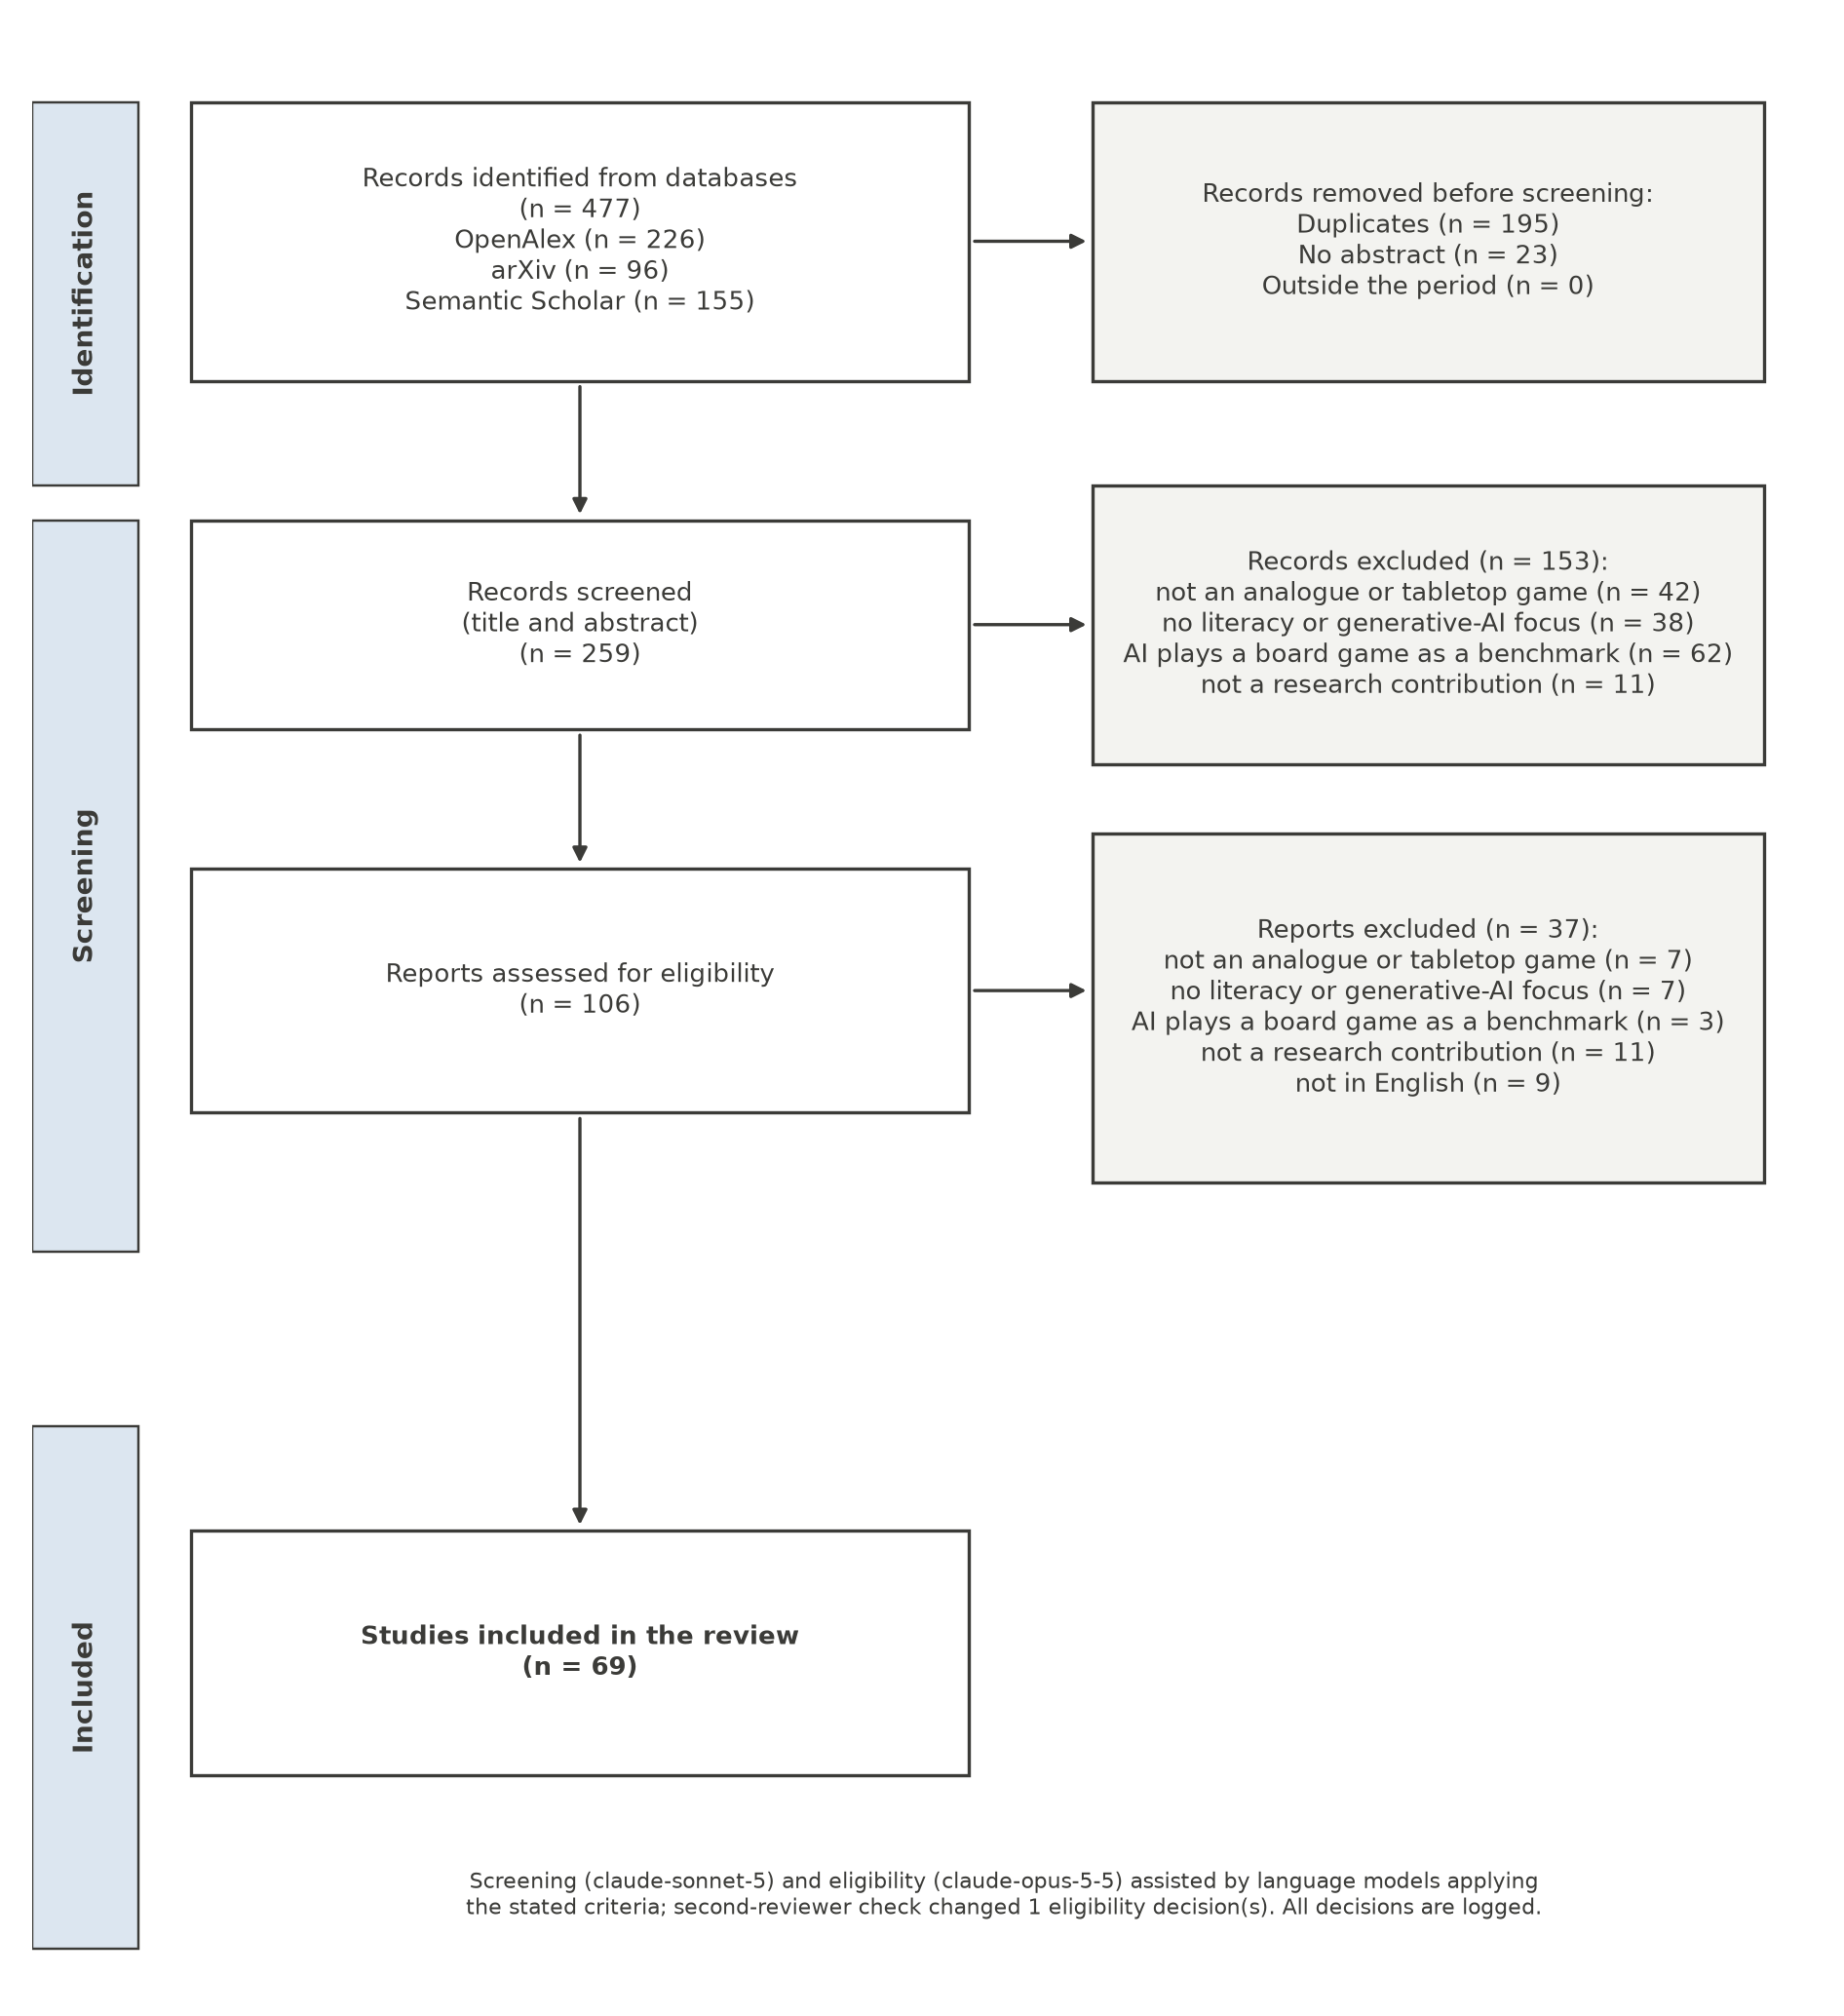
\includegraphics[width=0.78\textwidth]{prisma.png}
\caption{PRISMA 2020 flow diagram of the systematic review on analogue games
for media, information and AI literacy and on tabletop play with generative
AI.}
\label{fig:prisma}
\end{figure}

\emph{Analogue games for media, information and news literacy} (23 studies).
Board games have been designed to simulate real-world media dynamics in
media and information literacy workshops, evaluated from the perspective of
teachers and facilitators \parencite{revtab01} and with hundreds of students
\parencite{revtab02}; to simulate journalistic work and test effects on news
literacy and motivation \parencite{revtab03}; and to place players in a
simulated post-truth context \parencite{revtab42}. Quasi-experimental studies
report gains in learning achievement and flow \parencite{revtab57} and compare
competitive with cooperative play \parencite{revtab51}. Card games address
fake news directly \parencite{revtab59,revtab62}, and a board game based on
inoculation theory helped mothers resist misinformation about breastfeeding
\parencite{revtab68}.

\emph{Analogue games for AI literacy} (11 studies). Non-digital board and card
games teach AI concepts and ethics without devices: a family board game aimed
at lowering the digital divide \parencite{revtab20}, a card game in which
players audit the harms of AI products \parencite{revtab48}, an unplugged
card game on embeddings \parencite{revtab07} and a Turing-test role-play used
in a school without computers \parencite{revtab17}. A board game with
NFC-tagged pawns lets young children co-create stories with an AI
\parencite{revtab36}.

\emph{Generative AI in tabletop role-play} (26 studies). Most of this work
supports or replaces the game master: language models assist Dungeon Masters
with information and inspiration \parencite{revtab49}, act as game masters
\parencite{revtab52}, or are combined in multi-agent systems that reduce some
errors but introduce others, such as rule violations and spoilers
\parencite{revtab34}. Other systems replace players who leave the table
\parencite{revtab21}, or combine physical cards with generative AI that keeps
a group story coherent \parencite{revtab06}; design studies discuss how such
companions could change collaborative storytelling \parencite{revtab55}.

\emph{Generative AI in game design} (9 studies). Generative AI is also used to
design and adapt educational board games \parencite{revtab53}; in one case
study it reduced the teacher's workload \parencite{revtab39}.

\paragraph{Gap.} The media-literacy games in the review simulate media
dynamics and evaluate knowledge, attitudes, motivation or flow; none of the
abstracts describes a game whose spatial and informational rules let players
see how a shared account forms, or one that leaves an inspectable record of
it. The generative-AI studies focus on assisting or replacing the game
master; few combine physical play with AI characters at the same table, and
none uses that combination to compare how humans and AI relate events. The
board proposed here addresses these gaps.

% ---------------------------------------------------------------------
\section{The model}
% ---------------------------------------------------------------------

\subsection{The board as a matrix}

The board is a grid of $n \times n$ cells. Each cell is a passage, a barrier
or part of a \emph{place}; a place is a connected region of cells with a name
and a description, such as the warehouse, the customs house or the chapel
(Figure~\ref{fig:tabuleiro}). Two non-barrier cells are adjacent when they
share a side; hexagonal and eight-neighbour boards fit the same framework.
The board is therefore a graph $S = (C, A)$ whose vertices are cells, fully
described by its adjacency matrix $A$, with $A_{xy} = 1$ when cells $x$ and
$y$ are adjacent and $0$ otherwise.

Matrix powers answer the board's basic questions. Cell $y$ can be reached
from cell $x$ in at most $k$ steps when
\begin{equation}
  \left[(I + A)^k\right]_{xy} > 0,
\end{equation}
where $I$ is the identity matrix. A character that moves $m$ cells per turn
can therefore reach, in one turn, the cells where row $x$ of $(I + A)^m$ is
positive. Perception uses the same operator: a character at $x$ with
perception radius $r$ sees what happens in the cells $y$ for which
$[(I + A)^r]_{xy} > 0$, that is, the cells at most $r$ steps away. Bridges of
$S$ (passages whose removal disconnects the board) and articulation cells
(cells whose removal does so) are its chokepoints \parencite{tarjan1972}. The
places that many characters' premises mention are \emph{attractor places}.

\begin{figure}[t]
\centering
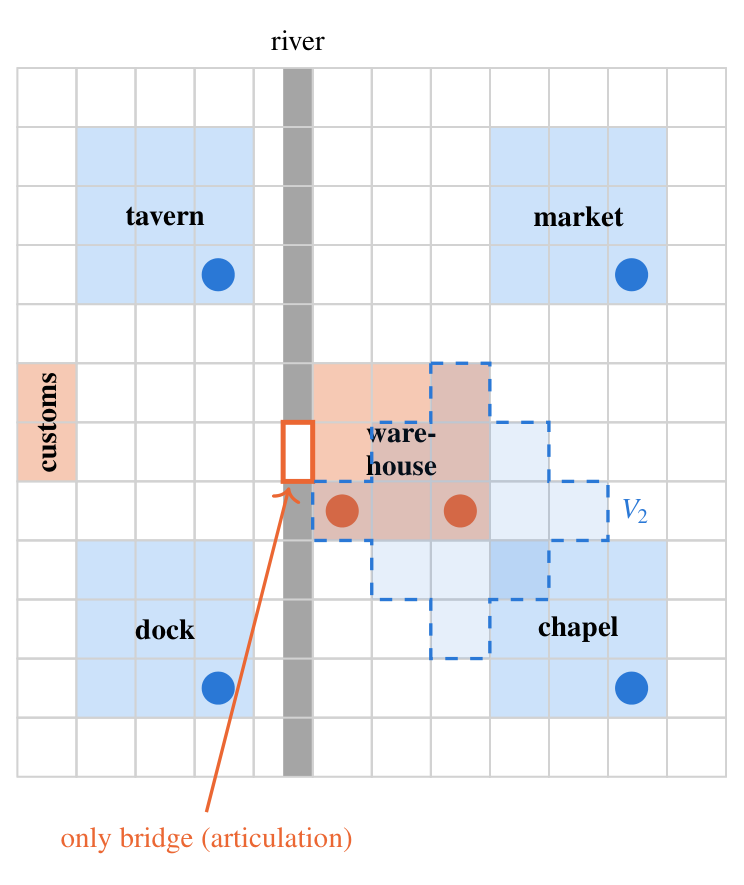
\includegraphics[width=0.55\textwidth]{tabuleiro.png}
\caption{An example board. Places are regions of cells; the warehouse and
the customs house are attractor places, named in several premises; a river
with a single bridge creates an articulation cell. Discs are characters; the
shaded cells are what one character sees with perception radius 2.}
\label{fig:tabuleiro}
\end{figure}

\subsection{Characters, encounters and knowledge}

Each character has a position on the board at every turn, a home place and
premises: an objective, a secret and two beliefs. Characters move toward
the places their premises make relevant. Two characters \emph{meet} at turn
$t$ when one is within the other's perception radius. Encounters form a
temporal network over the characters \parencite{holme2012}: let $M_t$ be the
encounter matrix at turn $t$, with $1$ for each pair of characters who meet.
Information can travel from character $a$ to character $b$ between turns
$t_0$ and $t_1$ only along a time-respecting path, which exists when
\begin{equation}
  R = \prod_{t=t_0}^{t_1-1}(I + M_t), \qquad R_{ab} > 0,
\end{equation}
with the product computed in Boolean arithmetic, so that $R_{ab}$ is
positive exactly when such a path exists. Each character holds a
\emph{knowledge set}: the events it caused, the events it saw and the events
it heard about from characters it met, each passed on with a rumour
probability $q$.

\subsection{Events and the causal graph}

Each turn, each character acts. The action becomes an event $v$ with an
author, a cell, a turn and a list of declared causes. The rule that defines
the model is that a character can only build on what it knows:
\begin{equation}
  u \in \mathrm{causes}(v) \;\Rightarrow\; u \in K_{\mathrm{author}(v)}\bigl(t(v)\bigr),
\end{equation}
where $K_a(t)$ is the knowledge set of character $a$ at turn $t$. For AI
characters the rule is enforced by prompting each character separately with
only its knowledge set; for people it is enforced by the physical kit.

The causal graph $G$ is built from the declared causes. Its connected
components are the \emph{storylines}, recomputed every turn: a storyline is
\emph{born} when a new component appears, \emph{fuses} when its events become
part of another storyline and \emph{closes} when it stops receiving new
events for three turns. The three graphs are nested
(Figure~\ref{fig:camadas}): the board $S$ bounds the encounters $H$, because
characters can only meet where the board lets them go, and $H$ bounds $G$,
because an event can only cite another if information about it could have
travelled to its author. This yields predictions that can be read off the
board before anyone plays: attractor places should concentrate the fusions;
chokepoints should be where separate storylines first meet; and storylines
started far apart should merge later.

\begin{figure}[t]
\centering
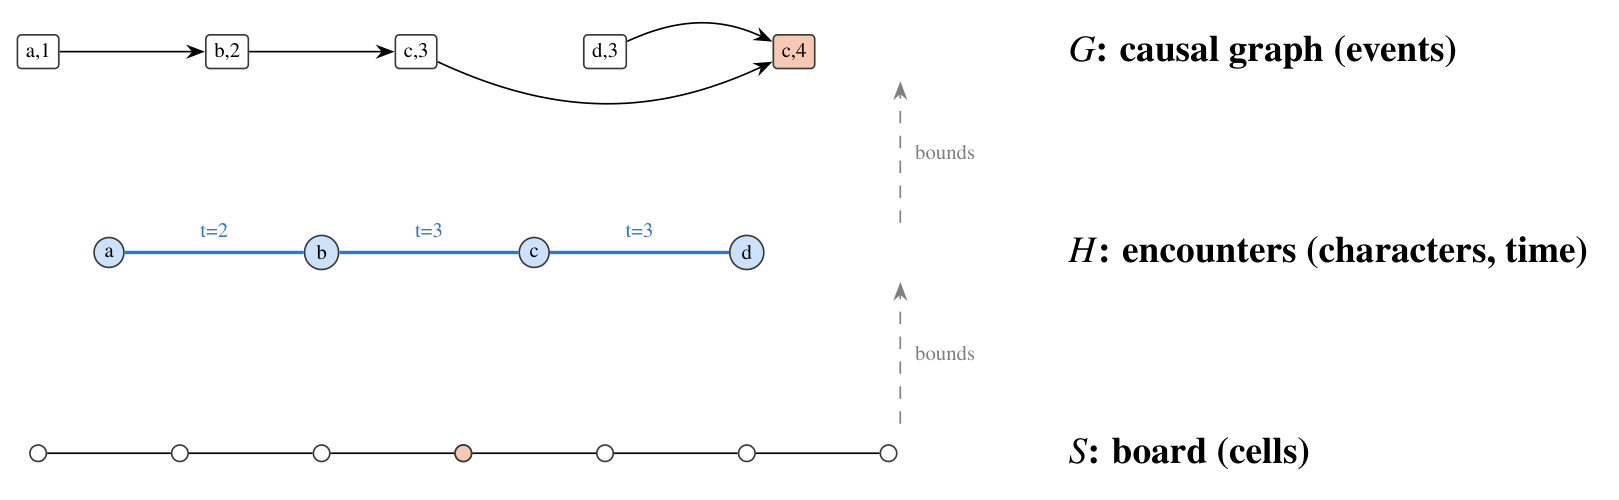
\includegraphics[width=\textwidth]{camadas.png}
\caption{The three layers. Where characters can go ($S$) bounds whom they
meet and when ($H$), which bounds what each event can cite ($G$). The
highlighted event, at an attractor place, merges two storylines.}
\label{fig:camadas}
\end{figure}

\subsection{What the model makes visible}

For media literacy, the value of the model is that it separates three things
that are usually confounded when people explain why a community believes
what it believes. The first is \emph{access}: who could have known about an
event, which is a property of space and encounters. The second is
\emph{uptake}: which known events a character chooses to build on, which is
a property of the character, human or AI. The third is \emph{structure}: the
shape of the resulting story, which emerges from the first two. A rumour that
spreads widely may do so because it was told in the place everyone passes
through, because those who heard it chose to repeat it, or because the
network had no other route. On the board, each of these explanations
corresponds to something that can be pointed at.

\subsection{A worked example}

A sequence from the companion study, generated by language-model agents in
the harbour town, shows what the board changes. On day 1, the merchant goes
to the warehouse to offer the widow a low price for it; the captain of the
guard orders some pages of the customs books set aside \enquote{before the
new inspector reads them}. On day 2, in the customs house, the merchant
offers the captain a purse to have the warehouse sealed for unpaid duties;
the captain accepts and has the pages rewritten; the inspector asks for the
books and notices the missing pages. On day 3 the captain seals the
warehouse, citing the bribe, his own acceptance and the inspector's inquiry,
and the merchant's and the captain's storylines become one.

In the omniscient simulator, every character could cite every one of these
events. On the board, each citation needs a route. The captain can cite the
bribe because he received it in person. Whether he can cite the inspector's
inquiry depends on whether he was in the customs house, or met someone who
was, before acting. The widow, who was at the warehouse on day 1 but not at
the customs house on day 2, cannot know about the bribe unless someone tells
her; if she later acts on it, the yarn will show who told her and where.
The same sequence, replayed on the board, thus produces a causal graph in
which every link has a visible explanation in space and time, and in which
the merger of the two storylines happens where the board says it can: in
the warehouse, the place the merchant's objective points to, where the
captain goes to seal it, made possible by what the two of them did in the
customs house the day before.

% ---------------------------------------------------------------------
\section{Proof of concept with synthetic agents}
% ---------------------------------------------------------------------

Before involving language models or learners, we asked which board mechanics
can change the convergence of a shared story at all. We wrote a minimal
simulation in which six synthetic characters move on a $12 \times 12$ board
with six places, two of them attractor places, and act once per day for 20
days. Each event cites a number of causes drawn from the distribution
observed with language-model agents in the companion study (mostly one or
two causes, almost never none), chosen at random among the recent events
the author \emph{knows}. The characters have no content and no intentions:
what is tested is the effect of structure alone.

We compared the omniscient regime of the existing simulator, in which every
character knows every recent event, with board regimes that vary the
perception radius, rumours and the presence of attractor places. We also
tested two design levers. \emph{Event cards} are two world events per day
that appear in random cells with no cause, such as a ship arriving or a
storm. The \emph{focus rule} requires that, in 80\% of actions, all causes
come from the same storyline, so that an action continues one thread rather
than tying several together. Each condition was run 500 times; the script
and its output are in the repository.

\begin{figure}[t]
\centering
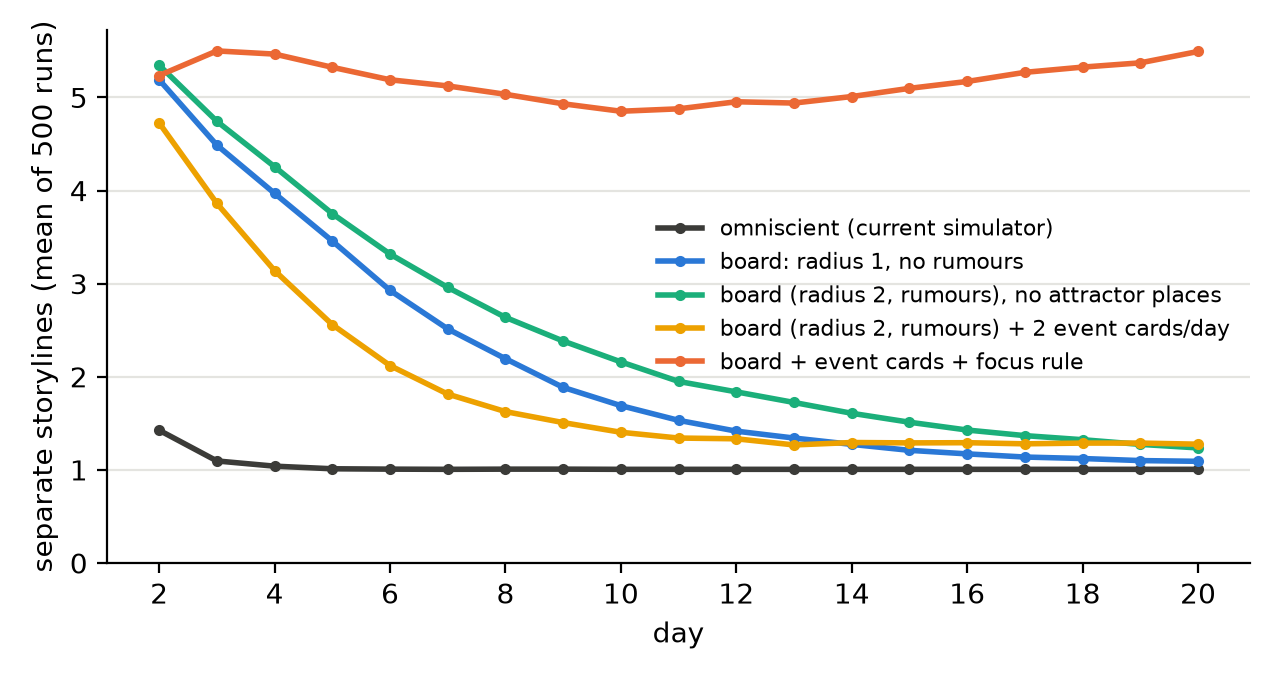
\includegraphics[width=0.85\textwidth]{linhas_por_condicao.png}
\caption{Separate storylines per day in the synthetic proof of concept, mean
of 500 runs per condition, 20 days.}
\label{fig:prova}
\end{figure}

\begin{table}[t]
\centering\small
\caption{Proof of concept with synthetic agents, 20 days, 500 runs per condition.}
\label{tab:prova}
\begin{tabularx}{\textwidth}{@{}Xrrrr@{}}
\toprule
Condition & Storylines at the end & Runs ending with one & Born after day 2 & Fusions near attractors \\
\midrule
Omniscient (current simulator) & 1.01 & 99\% & 0.1 & 91\% \\
Board, radius 2, rumours & 1.05 & 95\% & 0.0 & 85\% \\
Board, radius 1, no rumours & 1.09 & 91\% & 0.0 & 85\% \\
Board, radius 2, rumours, no attractor places & 1.24 & 79\% & 0.0 & 66\% \\
Board, radius 2, rumours, 2 event cards per day & 1.28 & 76\% & 1.3 & 86\% \\
Board, radius 2, rumours, event cards and focus rule & 5.49 & 2\% & 6.0 & 84\% \\
\bottomrule
\end{tabularx}
\end{table}

Three results stand out (Figure~\ref{fig:prova}, Table~\ref{tab:prova}).

\emph{Information changes the beginning, not the end.} In the omniscient
regime, the actions of the second day already cite each other across
characters, and only 1.5 storylines are born on average. On the board, each
character mostly knows its own past, and about five storylines are born, the
same order observed with language-model agents. But on every board without
further mechanics, almost all runs still end with a single storyline.
Reducing the perception radius or removing rumours only slows the process.
For teaching, this is the first lesson of the board: limiting who knows what
delays the formation of a single account, but does not prevent it as long as
everyone keeps building on what they know.

\emph{Attractor places decide where, and partly whether.} With attractor
places, more than 80\% of fusions happen next to them; without them, the
share falls to 66\% and one run in five keeps more than one storyline. The
places everyone needs are where separate accounts meet and merge.

\emph{New stories need new seeds and a reason not to knot.} Because every
character always knows its own past and almost always cites something, no
storyline is born after the second day unless the world supplies events
without causes. Event cards provide such seeds, but on their own they are
soon absorbed. Combined with the focus rule, they sustain five to six
storylines throughout the session, with new ones being born as others merge.
In media terms, plurality of accounts requires both new, independent sources
and a practice of not immediately connecting everything to the dominant
story.

Figure~\ref{fig:mesa} shows what these differences look like on the table
after eight turns of one run of each condition: with the board rules alone,
the yarn forms a single bundle around the attractor places; with world-event
cards and the focus rule, several bundles of different colours stay apart.

\begin{figure}[t]
\centering
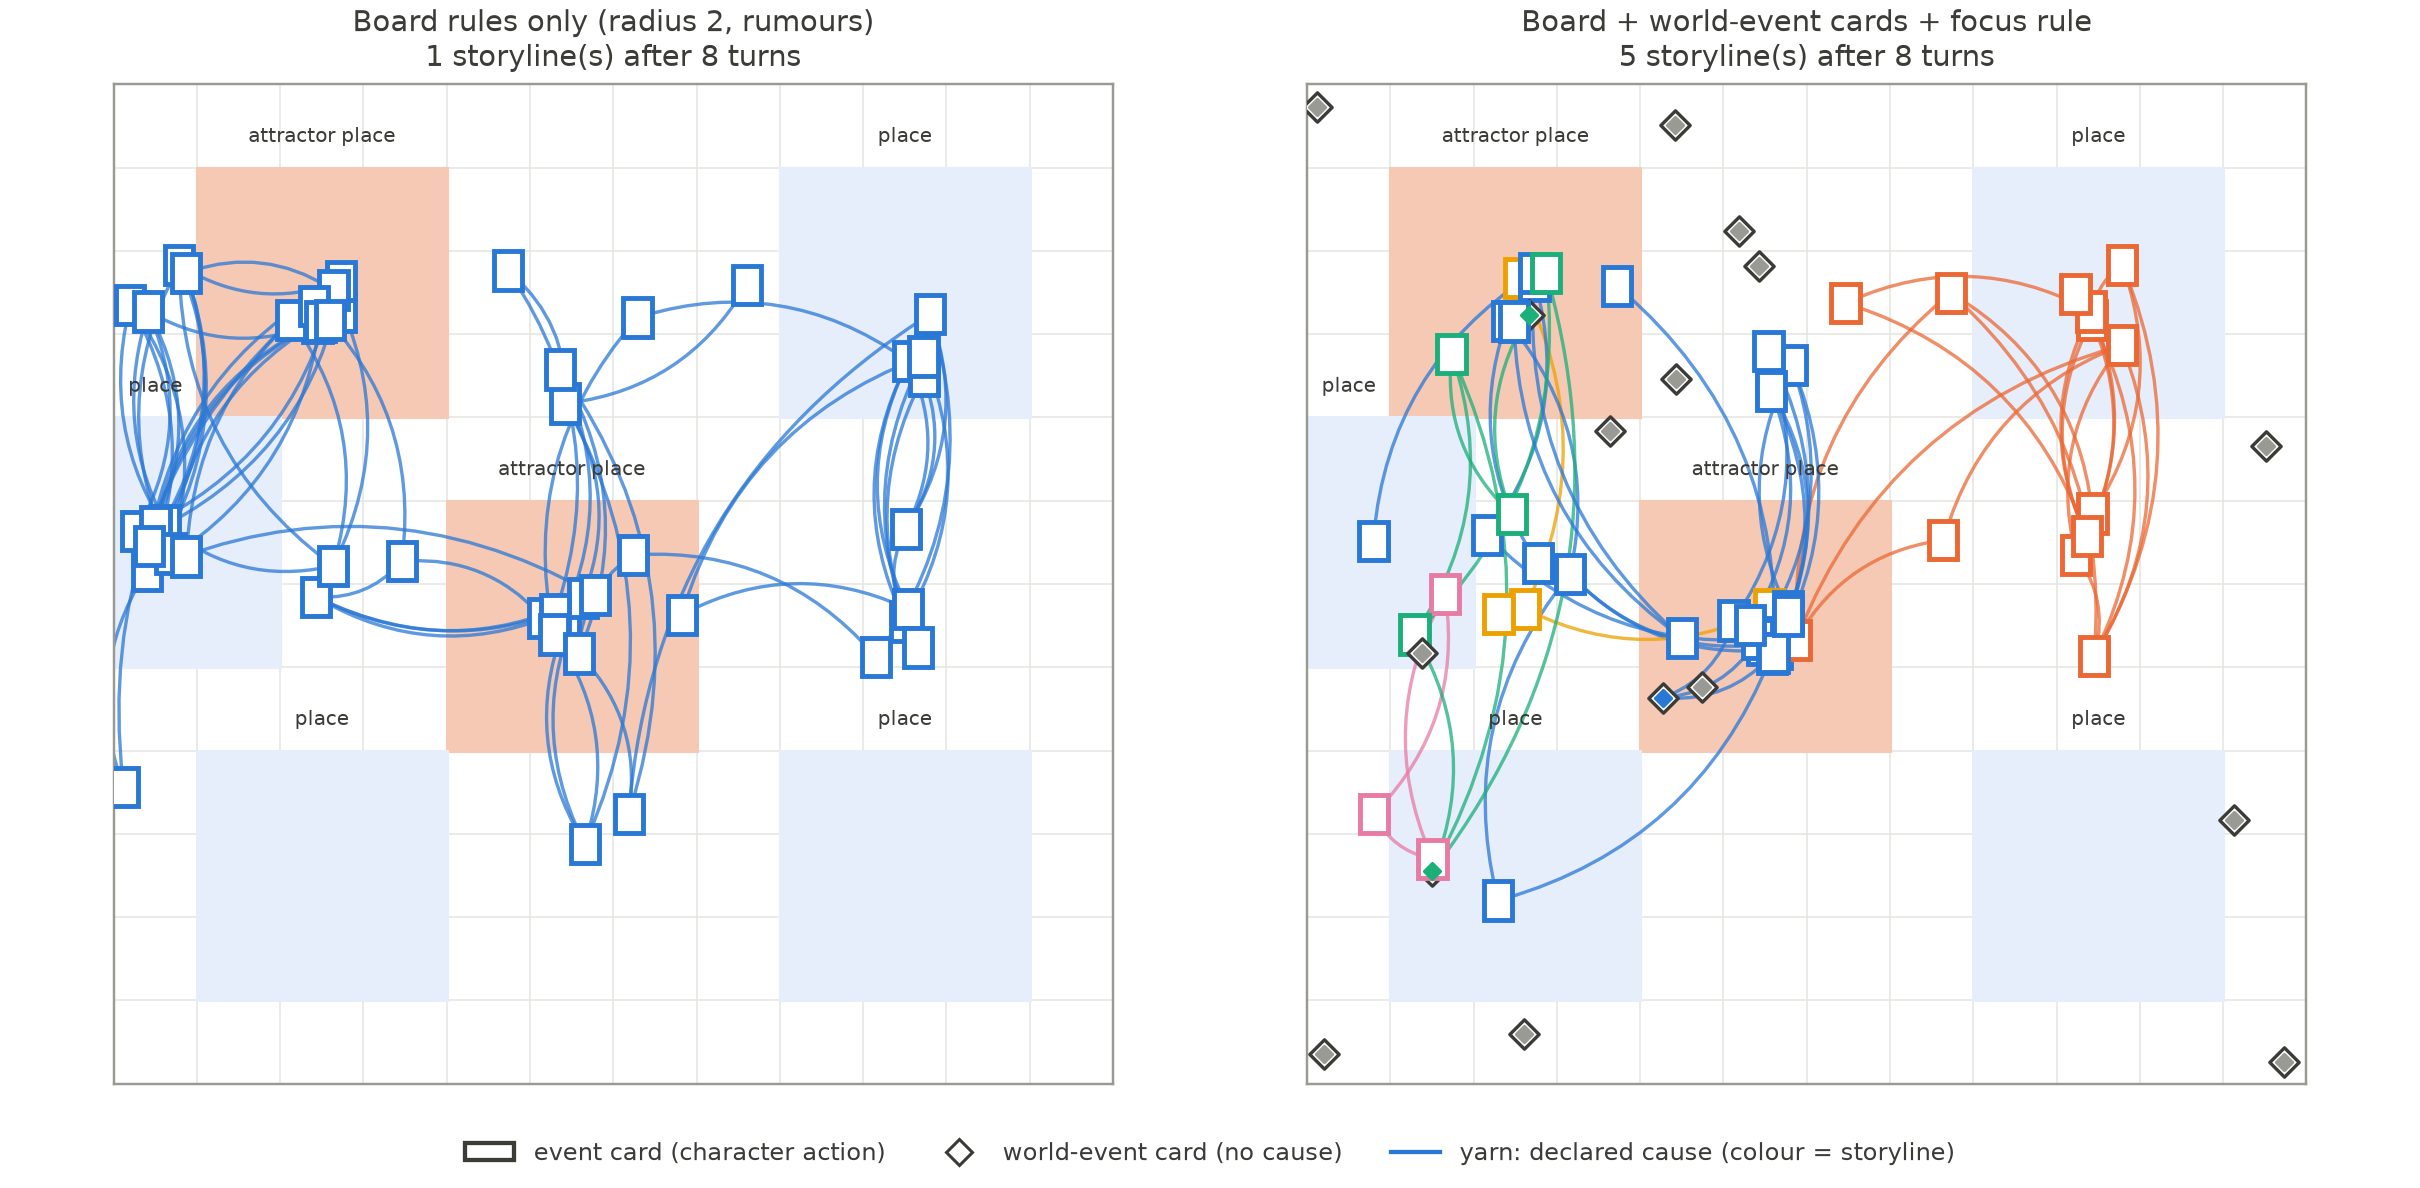
\includegraphics[width=\textwidth]{mesa.png}
\caption{The table after eight turns in one run of the synthetic proof of
concept, under two conditions. Rectangles are event cards placed on the cell
where they happened, diamonds are world-event cards, and lines are the yarn
between each card and the cards it cites, coloured by the storyline the card
belongs to at the end.}
\label{fig:mesa}
\end{figure}

The proof of concept has obvious limits: synthetic characters choose at
random and have no premises in the textual sense. Its value is to separate
what the board can do from what content does, and to tell us which mechanics
are worth taking to a classroom.

\subsection{From findings to mechanics}

Table~\ref{tab:mecanicas} summarises how each observation, from the
companion study or from the proof of concept, becomes a mechanic of the
board and a point for discussion in class.

\begin{table}[t]
\centering\small
\caption{From observations to board mechanics and learning points.}
\label{tab:mecanicas}
\begin{tabularx}{\textwidth}{@{}XXX@{}}
\toprule
Observation & Board mechanic & Learning point \\
\midrule
AI characters that see everything connect everything; storylines merge within days & Knowledge limited to what a character saw or heard; perception radius; rumours & Who \emph{could} have known: access shapes which accounts can meet \\
\addlinespace
Fusions happen in the places that several premises name & Attractor places on the board; chokepoints such as a single bridge & Central places and channels are where separate accounts merge \\
\addlinespace
No new storyline is born once every action cites the past & World-event cards with no cause & Plurality needs new, independent sources \\
\addlinespace
Limiting information only delays the merger & Focus rule: an action continues one thread & Norms of attribution and restraint keep accounts apart \\
\addlinespace
The story is invisible while it is being made & Yarn between event cards & The structure of a shared account can be inspected \\
\bottomrule
\end{tabularx}
\end{table}

% ---------------------------------------------------------------------
\section{The physical kit and the hybrid protocol}
\label{sec:kit}
% ---------------------------------------------------------------------

The same board is printed for a table of four to eight participants. The kit
contains the board, with places and a river; one token and one character
sheet per character, with objective, secret and beliefs; blank \emph{event
cards}, on which a player writes what the character does, the turn and the
identifier of each cause; coloured yarn, which connects each event card to
the cards it cites; a deck of world-event cards; and screens that hide each
player's known cards. Figure~\ref{fig:kit} shows the main components.

\begin{figure}[t]
\centering
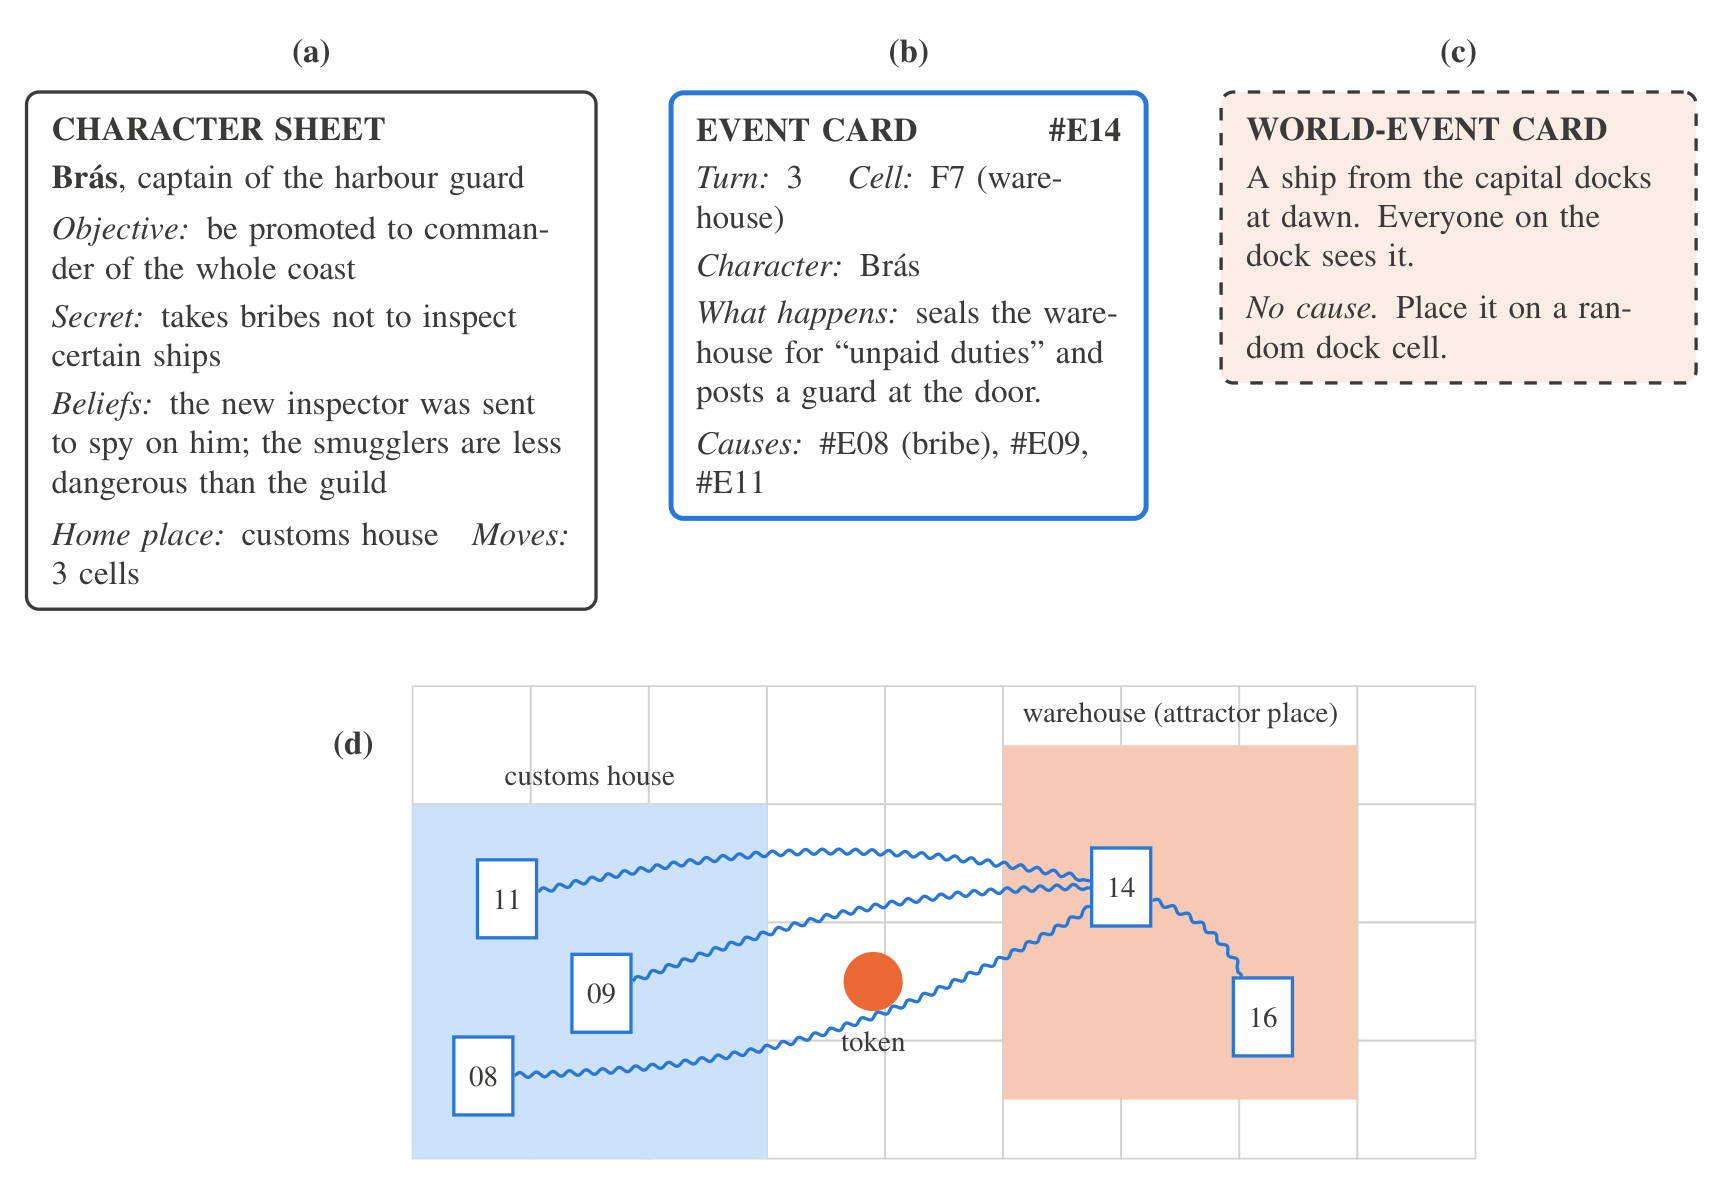
\includegraphics[width=\textwidth]{kit.png}
\caption{Components of the physical kit: (a) a character sheet with
objective, secret and beliefs; (b) an event card, with turn, cell, character,
action and the identifiers of the cards it cites; (c) a world-event card, which
has no cause; (d) on the table, each event card sits on the cell where it
happened and yarn ties it to the cards it cites. Card 14, in the warehouse,
cites three cards from the customs house: the yarn shows that its author could
only know about them because he was there.}
\label{fig:kit}
\end{figure}

A turn has four steps. First, characters move up to a fixed number of cells.
Second, the facilitator reveals world-event cards in the drawn cells. Third,
each player writes an event card and places it on the cell where it happens;
the card's causes must be cards the character knows, and the facilitator
ties the yarn. Fourth, knowledge is updated: a player adds to their hand the
cards placed within their token's perception radius, and players whose
tokens meet may show each other cards from their hands. Optional rules
switch the focus rule on or off, or change the radius and the number of
world-event cards. Varying these rules between rounds is part of the
learning design, as the classroom protocol below describes.

In hybrid tables, some characters are played by the simulator. The
facilitator, or a companion app, enters the AI characters' positions and
known cards; the simulator, prompting each character separately with only
its knowledge, returns the action and its causes, which are written on cards
like any other. Because every event card carries the same fields as the
simulator's event log, a photographed or transcribed table yields the same
data as a simulated session, and all analyses run unchanged on human, AI and
hybrid tables. At the end of the session the yarn \emph{is} the causal graph.

% ---------------------------------------------------------------------
\section{A classroom protocol}
\label{sec:aula}
% ---------------------------------------------------------------------

\subsection{Learning objectives}

The protocol targets four objectives, aligned with media literacy and AI
literacy frameworks \parencite{hobbs2010,long2020,unesco2024}:

\begin{enumerate}
\item explain how access to information, uptake and network structure each
contribute to the formation of a shared account;
\item identify, in a causal graph they built, the events and places through
which separate accounts merged;
\item compare how human and AI characters relate new events to past ones, and
recognise the tendency of generative models to connect everything they see;
\item propose and test changes to the rules of a community (more sources,
more routes, norms of attribution) that would preserve a plurality of
accounts.
\end{enumerate}

\subsection{A session of 100 minutes}

\emph{Preparation (10 minutes).} Groups of four to six receive the board and
a scenario. We use the two worlds of the companion study: a harbour town
with debt, bribery and smuggling, and a mountain village that must ration
grain before winter. Each student takes one character sheet. In hybrid
tables, one or two characters are played by the simulator.

\emph{First round (30 minutes).} Eight turns with the default rules: radius
2, rumours allowed, one world-event card per turn, no focus rule. The yarn
grows on the table as the story unfolds.

\emph{Prediction (10 minutes).} Before looking at the yarn as a graph, each
student writes how many separate stories they think the town has, which
character's account became dominant and why.

\emph{Reading the graph (20 minutes).} The group lifts the yarn and reads it
as a graph: which cards hold separate bundles together, at which place the
first bundles merged, whose stories were absorbed and never had their own
ending, and who knew what when. The facilitator asks the three questions
that correspond to the model: who \emph{could} have known this (access), who
\emph{chose} to build on it (uptake), and what would have happened without
this card or this place (structure).

\emph{Second round (20 minutes).} The group changes one rule and plays again:
adds world-event cards, adopts the focus rule, adds a second bridge, or
moves the place everyone needs. Students predict the effect before playing.

\emph{Debrief (10 minutes).} The discussion connects the board to media they
know: a group chat in which one message ties every conversation together, a
recommendation feed that routes everyone through the same few channels, or a
chatbot that, like the AI characters, connects whatever it is shown. The
closing question is what a community, or a platform, could change in its
rules to keep more than one account alive.

\subsection{The facilitator's role}

The facilitator, usually the teacher, does not narrate the story. Their role
is to keep the rules: checking that each card cites only cards its author
knows, tying the yarn, revealing world-event cards, and, in hybrid tables,
passing the AI characters' knowledge to the simulator and their actions back
to the table. This deliberately removes the figure of an omniscient game
master, whose presence would reintroduce the single point of view that the
board is meant to break. Preparation takes about an hour: printing the board
and the cards, reading the two scenarios, and, for hybrid tables, testing
the simulator with the chosen model. A short facilitator guide, with the
rules on one page and the debrief questions below, accompanies the kit.

\subsection{Debrief questions}

The facilitator can draw on a small bank of questions, grouped by the three
explanations the model separates.

\emph{Access.} Which cards could your character have seen? Who told you
about this event, where and when? Was there any story you never heard about
until the end? What would have changed if you had been on the other side of
the river?

\emph{Uptake.} Among the cards you knew, why did you build on these and not
others? Did you tie your card to the story everyone was following, or to your
own? Did the AI characters choose differently from the people at the table?

\emph{Structure.} Which card holds the largest bundle of yarn together? If
we cut it, how many stories would the town have? Which place appears most
often under the cards where bundles merge? Whose story was absorbed into
another one and never had its own ending, and why?

\emph{Transfer.} Where, in your own media use, is the \enquote{warehouse}
that everyone passes through? Which messages work like the card that ties
everything together? What rule would you add to a group chat, or to a
platform, to keep more than one account alive?

\subsection{A low-tech version}

The AI characters are optional. The full protocol runs with paper, yarn and
dice, which makes it usable in schools without devices or connectivity, a
concern of the call for this issue. In this version, the facilitator plays
one \enquote{connected} character who, unlike the others, sees every card on
the table and must cite at least two of them. This character reproduces, by
rule, the behaviour that the companion study observed in language-model
agents, and lets students discuss AI-like omniscience without using AI.

\subsection{Using generative AI with students}

Hybrid tables bring generative AI into the classroom, and with it questions
of privacy and control. The protocol is designed so that no personal data
reach the model: the AI characters receive only the fictional cards they
know, never students' names or writing beyond the event cards of the game.
The simulator also runs with open models on a local machine, which avoids
sending any classroom content to an external service and keeps the activity
possible where commercial services are restricted. The teacher decides which
characters, if any, are played by AI, and every AI action passes through the
facilitator before it becomes a card on the table, so the model never
addresses students directly. Finally, the AI characters are presented as what
they are, programs that write plausible actions from what they are given,
which is itself part of the learning objective: students compare how these
characters relate events with how they themselves do.

\subsection{Accessibility}

Cards can be printed in large type and read aloud; tokens can carry tactile
marks; and the number of turns can be reduced for younger players. Writing an
event card can be replaced by telling it to a scribe. The board's logic
does not depend on reading speed, which makes it suitable for mixed groups.

% ---------------------------------------------------------------------
\section{Evaluation plan}
% ---------------------------------------------------------------------

We plan two studies, to be pre-registered with the same procedures as the
companion study \parencite{nosek2018}.

\emph{Study 1: simulation with language-model agents.} The existing simulator
will be extended with the board and with per-character prompts restricted to
knowledge sets. With the same worlds and models as the companion study, we
will cross the omniscient and board regimes, the perception radius, rumours,
event cards and the focus rule. Hypotheses: (H1) on the board, more
storylines are born and fusions happen later than in the omniscient regime;
(H2) fusions concentrate at attractor places and chokepoints; (H3) without
event cards, no storylines are born after the first days; (H4) event cards
with the focus rule sustain several storylines and allow closures.

\emph{Study 2: classroom sessions.} Upper-secondary and first-year university
classes will play the protocol in three formats: human only, hybrid, and
human only with the \enquote{connected} character of the low-tech version.
Measures include the graph metrics of each table; the written predictions
and explanations, coded for references to access, uptake and structure; and a
short pre/post instrument on how participants explain the formation of shared
accounts in a news scenario. Hypotheses: (H5) human tables cite fewer causes
per event than AI characters and keep more storylines separate; (H6) after
reading the graph, students refer more often to access and structure, not
only to individual intentions, when explaining why an account became
dominant; (H7) the second round, with rules chosen by the students, keeps more
storylines alive than the first. Studies with students will follow the
ethics procedures of the authors' institution, with informed consent from
students and guardians, and anonymised data.

% ---------------------------------------------------------------------
\section{Discussion}
% ---------------------------------------------------------------------

The board is a small model of a question at the heart of media literacy:
how a community comes to share one version of events. Its main contribution
is to make the structure of that process tangible and inspectable. Students
who see their character's story absorbed into someone else's, because they
were on the wrong side of the river or never heard the rumour, experience
how access to information and to central places translates into narrative
power; and the yarn graph gives them an object to reason about it with.

The proof of concept qualifies a common intuition. One might expect that
limiting who knows what, the board's basic rule, would be enough to keep
several accounts alive. It is not: as long as every participant keeps
building on what they know, the accounts eventually meet. What preserves
plurality is the combination of new independent sources and a norm of not
tying every new event to the dominant story. Both have recognisable
counterparts in information ecosystems: diversity of sources, and practices
of attribution and restraint in sharing. The board lets students discover
this by changing the rules and seeing the graph change.

The hybrid format adds a dimension that is specific to generative AI. The
companion study found that language-model agents almost never act without
citing something that already happened, and the low-tech \enquote{connected}
character turns that observation into a rule anyone can play. Comparing
human and AI characters at the same table makes visible a property of these
systems that is hard to see in a single conversation: their tendency to
connect whatever they are shown, and with it, to pull separate stories into
one.

\subsection{Limitations}

The model is a design proposal with a proof of concept, not an evaluated
intervention. The proof of concept uses synthetic characters and says nothing
about the content that language models or students would produce on the
board. The formal model treats knowledge as sets of events, a simplification
of what people believe, forget and misremember. The physical kit has not yet
been playtested; its turn structure may be heavy for some groups, and a
digital companion may be needed to manage knowledge in larger classes. The
classroom protocol and its measures are proposals whose validity must be
established in the planned studies.

% ---------------------------------------------------------------------
\section{Conclusion}
% ---------------------------------------------------------------------

Representing the world of a role-playing game as a board, and the board as
a matrix, makes it possible to reason about a shared story with the tools of
graph theory: the board bounds the encounters, the encounters bound the
causal graph, and the causal graph is the story. A simulation shows that the
board alone does not prevent a shared story from collapsing into one, that
central places decide where it collapses, and that new sources together with
a norm of focus keep several stories alive. Played with paper and yarn, with
or without AI characters, the same board turns this structure into something
a class can see, discuss and change: how space, information and power decide
which story a community ends up telling.

\section*{Data and code availability}
The simulation script, its results and the sources of the figures are
available in a public repository [link removed for review].

\printbibliography

\end{document}
